% Roll, pitch, yaw rotations about x, y, z
\documentclass[dvisvgm,tikz,border=4pt]{standalone}
% Shared preamble for the TikZ figures in images-1/src (compiled by build.sh)
\usepackage{helvet}
\renewcommand\familydefault{\sfdefault}
\usepackage{amsmath, amssymb}
\usetikzlibrary{arrows.meta, calc, decorations.pathreplacing, patterns, positioning, shapes.geometric, 3d, perspective, fit, backgrounds}
% palette shared with slides.scss and the Graphviz diagrams
\definecolor{dmred}{HTML}{880000}
\definecolor{dmblue}{HTML}{000088}
\definecolor{dmgreen}{HTML}{008800}
\definecolor{dmorange}{HTML}{E08A1E}
\definecolor{ink}{HTML}{333333}
\definecolor{fillblue}{HTML}{E8E8F8}
\definecolor{fillred}{HTML}{F3EAEA}
\definecolor{fillgreen}{HTML}{E8F4E8}
\definecolor{fillorange}{HTML}{FDF0DC}
\definecolor{steel}{HTML}{C9D3DC}
\definecolor{steeldk}{HTML}{8FA3B5}
\definecolor{metal}{HTML}{D9D9D9}
\definecolor{metaldk}{HTML}{A6A6A6}
\tikzset{
  >={Stealth[length=7pt]},
  every picture/.style={line cap=round, line join=round, font=\large},
  proj/.style={gray, dashed, thin},
  dim/.style={<->, >={Stealth[length=5pt]}, thin},
  ext/.style={very thin, gray},
  callout/.style={gray!70!black, thin},
  % datum (origin) symbol
  % pics use absolute sizes so they look the same in mm-scaled drawings
  datum/.pic={
    \fill[white] (0,0) circle (0.22cm);
    \fill[black] (0,0) -- ++(0.22cm,0) arc[start angle=0, end angle=-90, radius=0.22cm] -- cycle;
    \fill[black] (0,0) -- ++(-0.22cm,0) arc[start angle=180, end angle=90, radius=0.22cm] -- cycle;
    \draw[thick] (0,0) circle (0.22cm);
  },
  % reference symbols (absolute sizes): origins have a double circle with a filled quadrant
  wporigin/.pic={
    \draw[thick, fill=white] (0,0) circle (0.3cm);
    \fill[black] (0,0) -- (0.18cm,0) arc[start angle=0, end angle=-90, radius=0.18cm] -- cycle;
    \draw[thick] (0,0) circle (0.18cm);
    \draw (-0.3cm,0) -- (0.3cm,0) (0,-0.3cm) -- (0,0.3cm);
  },
  machorigin/.pic={
    \draw[thick, fill=white] (0,0) circle (0.3cm);
    \fill[black] (0,0) -- (-0.18cm,0) arc[start angle=180, end angle=90, radius=0.18cm] -- cycle;
    \draw[thick] (0,0) circle (0.18cm);
    \draw (-0.3cm,0) -- (0.3cm,0) (0,-0.3cm) -- (0,0.3cm);
  },
  supportpt/.pic={
    \draw[thick, fill=white] (0,0) circle (0.15cm);
    \draw (-0.15cm,0) -- (0.15cm,0) (0,-0.15cm) -- (0,0.15cm);
  },
  regpt/.pic={
    \draw[thick, fill=white] (0,0) circle (0.24cm);
    \draw[thick] (0,0) circle (0.15cm);
    \draw (-0.15cm,0) -- (0.15cm,0) (0,-0.15cm) -- (0,0.15cm);
  },
  % support / registration point (generic)
  target/.pic={
    \draw[thick, fill=white] (0,0) circle (0.12cm);
    \draw (-0.2cm,0) -- (0.2cm,0) (0,-0.2cm) -- (0,0.2cm);
  },
}

\begin{document}
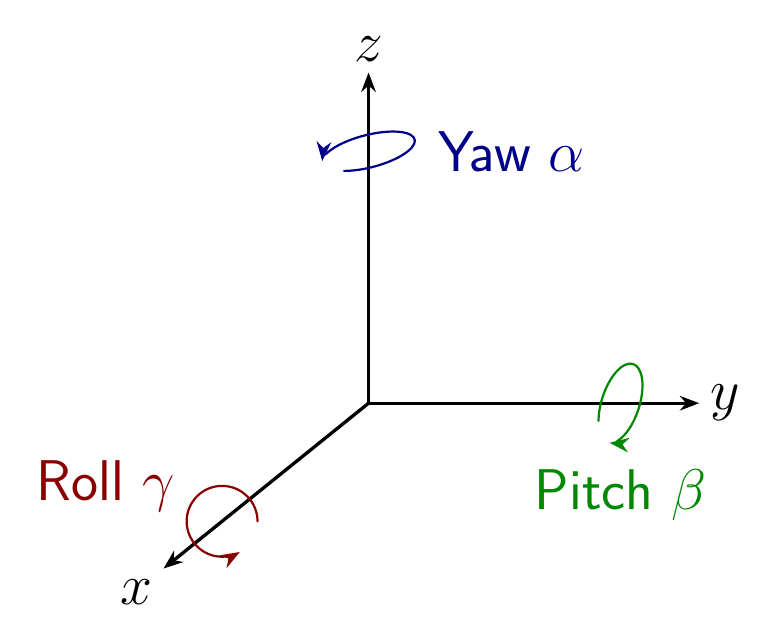
\begin{tikzpicture}[x={(-0.62cm,-0.5cm)}, y={(1cm,0cm)}, z={(0cm,1cm)}, font=\huge, line width=1.2pt]
  \draw[->, very thick] (0,0,0) -- (4.2,0,0) node[below left] {$x$};
  \draw[->, very thick] (0,0,0) -- (0,4.2,0) node[right] {$y$};
  \draw[->, very thick] (0,0,0) -- (0,0,4.2) node[above] {$z$};
  % rotation arrows: circles in the plane normal to each axis
  \begin{scope}[canvas is yz plane at x=3.0]
    \draw[->, thick, dmred] (0:0.45) arc[start angle=0, end angle=300, radius=0.45];
  \end{scope}
  \begin{scope}[canvas is xz plane at y=3.2]
    \draw[->, thick, dmgreen] (0:0.45) arc[start angle=0, end angle=300, radius=0.45];
  \end{scope}
  \begin{scope}[canvas is xy plane at z=3.2]
    \draw[->, thick, dmblue] (0:0.5) arc[start angle=0, end angle=300, radius=0.5];
  \end{scope}
  \node[dmred, anchor=east] at (2.3,-0.9,0.1) {Roll $\gamma$};
  \node[dmgreen, anchor=north]     at (0,3.2,-0.7)   {Pitch $\beta$};
  \node[dmblue, anchor=west]       at (0,0.75,3.2)   {Yaw $\alpha$};
\end{tikzpicture}
\end{document}
